\documentclass{uflamon}          % classe base para a monografia

%==============================================================================
% Utilizacao de pacotes
\usepackage{float}
\usepackage[T1]{fontenc}         % usa fontes postscript com acentos
\usepackage[brazil]{babel}       % hifenização e títulos em português do Brasil
\usepackage[utf8]{inputenc}     % permite edição direta com acentos
\usepackage{amsmath}             % pacote da AMS para Matemática Avançada
\usepackage{amssymb}             % símbolos extras da AMS
\usepackage{latexsym}            % símbolos extras do LaTeX
\usepackage{graphicx}            % para inserção de gráficos
\usepackage{listings}            % para inserção de código
\usepackage{fancyvrb}            % para inserção de saídas de comandos
%\usepackage{enumerate}           % para personalizar lista enumeradas 
											%(incluso na classe)
\usepackage{longtable}           % para tambelas muito grandes NOVO!!!!

\usepackage{colortbl} % cores em tabelas
\newcolumntype{Z}{|>{\columncolor[gray]{0.9}}l|} %cor cinza em células
%\usepackage{array} % já incluso na classe
\newcolumntype{L}[1]{>{\raggedright\let\newline\\\arraybackslash\hspace{0pt}}m{#1}}
\newcolumntype{C}[1]{>{\centering\let\newline\\\arraybackslash\hspace{0pt}}m{#1}}
\newcolumntype{R}[1]{>{\raggedleft\let\newline\\\arraybackslash\hspace{0pt}}m{#1}}
\usepackage{multirow} % para juntar duas linhas em uma só

\usepackage{multicol} % para uso de várias colunas

% cores para os links cruzados
\usepackage{color}
\definecolor{rltred}{rgb}{0.2,0,0}
\definecolor{rltgreen}{rgb}{0,0.2,0}
\definecolor{rltblue}{rgb}{0,0,0.2}

\usepackage[colorlinks=true,
            urlcolor=rltblue,       % \href{...}{...} external (URL)
            filecolor=rltgreen,     % \href{...} local file
            linkcolor=rltred,       % \ref{...} and \pageref{...}
            citecolor=rltgreen,
            pdftitle={Exemplo de Uso da Classe Uflamon},
          pdfauthor={Joaquim Quinteiro Uchôa},
          pdfsubject={Este texto tem por objetivo servir de exemplo da classe Uflamon.},
          pdfkeywords={Comunicação Científica. 2. Pesquisa . 3. Pesquisa Científica. 
 					 4. Redação. 5. Monografia.}%
]{hyperref} % para referência cruzadas
%\usepackage{hyperref}            % para referência cruzadas
\usepackage{subfigure}           % figuras dentro de figuras
\usepackage{caption}            % remodelando o formato dos títulos de 
                                 % tabelas e figuras

% configuração padrão do listings   
\lstset{
   language=Java,
   extendedchars=true,
   tabsize=3,
   basicstyle=\footnotesize\ttfamily,
   stringstyle=\em,
   showstringspaces=false 
}

% para referências de acordo com a ABNT
% precisa instalar o abntex2 antes!!!
% http://abntex.codigolivre.org.br/
% comente se pretende usar outro padrão

%abnt-emphasize=bf coloca o título das bibliografias em negrito
%abnt-thesis-year=both
\usepackage[alf,abnt-etal-cite=3,abnt-etal-list=3,abnt-url-package=url,abnt-emphasize=bf]{abntex2cite}

% evite usar o hyperref com abntex, pode dar caca em urls... no linha anterior, informo
% para incluir urls usando o pacote url e não o hyperref
%
% caso queira o hyperref com abntex, comente a linha anterior e descomente a seguinte
%\usepackage[alf,abnt-etal-cite=3,abnt-etal-list=0,abnt-etal-text=emph]{abntex2cite}
%
% caso vc ainda use a versão anterior da abntex, comente a linha incluindo o abntex2cite
% e descomente a próxima linha 
%\usepackage[alf,abnt-etal-cite=3,abnt-etal-list=0,abnt-etal-text=emph]{abntcite}


% redefinindo formatação de títulos de tabelas e figuras


%==============================================================================
% para os fãs do Word, descomente as linhas abaixo
%\sloppy %mais espaço entre as linhas
%\usepackage{identfirst} %identando-se a primeira linha de cada seção
%\noindentfirst % Tire o comentário para manter o padrão do LaTeX.

%==============================================================================
% definido comandos na monografia - não é necessário na sua monografia 
% apenas para exemplificar a definição de novos comandos
\newcommand{\defs}[1]{\textsl{#1}}


% Especificando hifenizações que por ventura LaTeX não saiba fazer
% Por padrão 99,9% dos termos em português devem ser hifenizados corretamente.
\hyphenation{hardware software Li-nux am-bien-te diag-nos-ti-car coor-de-na-ção 
FAE-PE Recovery TelEduc Williams UFLA}

%==============================================================================
% Dados da monografia, capa: autor, titulo, banca, etc... - SUBSTITUA DE ACORDO
%==============================================================================
\author{Lucas Fonseca dos Santos}
\title{Análise da viabilidade da aplicação de soluções em processamento de línguas naturais para idioma português.}
%\subtitle{Relatório Final}
%\engtitle{Relatório Final}
%\engsubtitle{Sample for Users}
\edicao{Programa  Voluntário de  Iniciação  Científica  (PVIC).}
\date{2018}
\tipo{Relatório de projeto do Programa Voluntário de Iniciação Científica (PVIC) apresentado a Universidade Federal de Lavras (UFLA).}
% use \orientador ou \orientadora quando for o caso
%\orientador{}
\orientadora{Prof. Juliana Galvani Greghi}
% use \coorientador ou \coorientadora quando for o caso
%\coorientadora{Prof. DSc. Maria Orientadora } % comente se não tiver coorientador
%\coorientador{}
\local{Lavras -- MG}
%\bancaum{Prof. MSc. Antônio Banca Um}{UFM}
%\bancadois{Prof. DSc. João Banca Dois}{FCO} % comente se sua banca tiver só um professor
%\bancatres{Profa. Esp. Eliza Banca Três}{BELMIS}
%\bancaquatro{Prof. Esp. Carlos Banca Quatro}{IBGPLUS}
%\defesa{30 de Fevereiro de 2016}
%==============================================================================

%\antesfichacat{\noindent Para citar este documento: \\UNIVERSIDADE FEDERAL DE LAVRAS. Biblioteca Universitária. \textbf{Manual de normalização e estrutura de trabalhos acadêmicos: TCC, monografias, dissertações e teses}. 2. ed. rev., atual. e ampl. Lavras, 2015. Disponível em: \url{http://www.biblioteca.ufla.br/wordpress/wpcontent/uploads/bdtd/manual_normalizacao_UFLA.pdf}. Acesso em: data de acesso.}

%\depoisfichacat{\noindent A reprodução e a divulgação total ou parcial deste trabalho são autorizadas, por qualquer meio convencional ou eletrônico, para fins de estudo e pesquisa, desde que citada a fonte.\\
%\newline
%{\small Este documento possui páginas em branco para facilitar a impressão frente-e-verso.}}

%##################################################

%##################################################

% para os exemplos do manual
%\newenvironment{exemplomanual}{
%\vspace{0.5cm}
%\noindent\begin{minipage}{\textwidth}
%\noindent\rule{\textwidth}{0.5pt}
%\vspace{-1cm}
%\begin{flushleft}
%}{
%\end{flushleft}
%\vspace{-0.6cm}
%\noindent\rule{\textwidth}{0.5pt}
%\vspace{0.3cm}
%\end{minipage}
%}

%\newenvironment{exemplomanuallista}{
%\vspace{0.3cm}
%\noindent\begin{minipage}{\textwidth - 0.5cm}
%\noindent\rule{\textwidth}{0.5pt}
%\vspace{-1cm}
%\begin{flushleft}
%}{
%\end{flushleft}
%\vspace{-0.6cm}
%\noindent\rule{\textwidth}{0.5pt}
%\vspace{0.3cm}
%\end{minipage}
%}

% por conta de alguns exemplos
%\usepackage{setspace}

%##################################################

% se vc já defendeu e tem o arquivo escaneado da folha de rosto, 
% descomente e altere o nome do arquivo
%\folhaAprovacaoAssinada{folharosto}

% Aqui começa o documento propriamente dito
\begin{document}

\maketitle

%\dedic{Espaço reservado a dedicatória.}     % Dedicatórias\\

%\thanks{Espaço reservado aos agradecimentos.}         % Agradecimentos

%\epigrafe{ % citação opcional

% palavras-chave
\keywords{Natural Language. Model Generation. Test Model. Requirement Document. Information Extraction. State Model. State Machine. Automaton Test. Automaton Generation.}
\resumo{Ao logo dos anos, tem sido percebido o aumento no número de empresas da área de tecnologia da informação que passaram a considerar a importância dos processos de testes de software como meio de aumento da qualidade dos produtos finais e redução de problemas decorrentes de falhas humanas e/ou falhas inerentes ao processo de desenvolvimento de sistemas computacionais.

Para tal questão, expandiu-se nos últimos anos a quantidade de ferramentas que auxiliam as empresas nesse processo, dentre as quais, podem ser citadas as ferramentas capazes de interpretar documentos de requisitos em língua natural estruturada, objetivando a geração de modelos de teste de forma mais mecanizada e automática. Várias pesquisas já foram publicadas a esse respeito, sendo a grande maioria para documentos de requisitos em língua inglesa.

O atual cenário de ferramentas dessa natureza demonstra que existem poucas opções disponíveis no mercado, sendo a grande maioria fruto de pesquisas acadêmicas e que ainda não foram amplamente divulgadas e disponibilizadas. Outro fator que dificulta o acesso às ferramentas é o idioma em que os documentos são expressos.

Esta pesquisa teve como objetivo a identificação e  análise das soluções já existentes, buscando identificar a viabilidade de sua aplicação para o idioma português e os resultados dessa aplicação. Tal processo de análise envolveu revisões da literatura e testes práticos com ferramentas de Processamento de Línguas Naturais (PLN).

Durante o desenvolvimento da pesquisa foi identificado que as técnicas de etiquetação e análise sintática são essenciais e, por não existirem muitas opções de ferramentas gratuitas para o tratamento da língua portuguesa, estão sendo analisadas as possibilidades de desenvolvimento de ferramentas próprias ou a adoção de ferramentas que façam o tratamento parcial das informações. Foram selecionados trabalhos relevantes, que servirão de inspiração para o desenvolvimento de uma ferramenta para automatização da geração de modelos de teste para a língua portuguesa. 

Como resultado da pesquisa desenvolvida até o momento, pode-se perceber que é viável a construção de uma ferramenta dessa natureza para documentos em língua portuguesa e que, sendo desenvolvida seguindo a filosofia do software livre, esta poderia auxiliar empresas de pequeno e médio porte, que também sofrem com problemas na produção de sistemas computacionais, e que podem ter menos capital para investimento em processos de teste eficientes e eficazes.}  % Resumo (digite aqui o resumo)

% keywords devem vir antes do abstract
\keywords{Natural Language. Model Generation. Test Model. Requirement Document. Information Extraction. State Model. State Machine. Automaton Test. Automaton Generation.} % keywords
\abstract{At the turn of the century, it has been noticed the increase in the number of companies in the area of information technology that have come to consider the importance of software testing processes as a means of increasing the quality of the final products and reducing problems arising from human and / or failures inherent to the process of development of computational systems.

To this end, the number of tools that help companies in this process has expanded in recent years, among which, the tools capable of interpreting requirements documents in a structured natural language can be cited, aiming the generation of test models in a way more mechanized and automatic. Several researches have already been published on this subject, most of which are for English language requirements documents.

The current scenario of tools of this nature shows that there are few options available in the market, most of which are the result of academic research and have not yet been widely disseminated and made available. Another factor that hinders access to tools is the language in which documents are expressed.

The objective of this research was to identify and analyze the existing solutions, seeking to identify the feasibility of its application to the Portuguese language and the results of this application. This analysis process involved literature reviews and practical tests with Natural Language Processing (PLN) tools.

During the development of the research it was identified that the techniques of tagging and syntactic analysis are essential and, because there are not many free tool options for the treatment of the Portuguese language, the possibilities of developing own tools or the adoption of tools that partial treatment of the information. Relevant works were selected, which will serve as inspiration for the development of a tool for automating the generation of test models for the Portuguese language.

As a result of the research developed so far, one can see that it is feasible to construct such a tool for documents in Portuguese language and that, being developed following the philosophy of free software, this could help small and medium-sized companies, who also suffer from problems in the production of computer systems, and which may have less capital to invest in efficient and effective testing processes.}

%##################################################

% Dados do guia
%\begin{titlepage}
%\pagestyle{empty}
%\renewcommand{\baselinestretch}{1}
%\enlargethispage{1.5cm}
%\input{reitoria}
%\cleardoublepage
%\end{titlepage}

%##################################################

% descomente para habilitar a lista desejada
\listoffigures                             % Lista de Figuras
%\listofilustracoes
%\listofgraficos							   % Lista de Gráficos
\listoftables                              % Lista de Tabelas
\listofquadros							   % Lista de Quadros
%\listofexemplos
%\listofteoremas
\tableofcontents                           % Sumário

\clearpage

\pagestyle{ufla}

%==============================================================================
% incluindo os capitulos
\chapter{INTRODUÇÃO}
\label{cap:introdução}

Este catapítulo apresenta uma visão geral do problema pesquisado bem como as soluções encontradas para tal, juntamente com os materiais e metologias empregados na busca da solução.

\section{Justificativa}

\subsection{Introdução a Teste de Software}
A construção de softwares em ampla maioria dos casos, usufruem dos planejados e estudados processos da engenharia de software objetivando uma escalabilidade desse processo para tentar se evitar erros, seja na implementação técnica dos algorítimos ou em errôneas interpretações casuais por parte de analises humanas equivocadas. Existem diversas técnicas para testes de software, mas em sua generalidade, trabalham sobre a ideia de avaliar dado um conjunto de possíveis entradas, a saída processada de tais conjuntos através das permutações de estados que o software em questão pode assumir.

Denota-se um problema intratável avaliar todas as possíveis entradas para um software, haja visto a cardinalidade de certos conjuntos de entrada, então, muitas técnicas exprimem a estratégia de se selecionar subconjuntos contidos no conjunto de entradas possíveis, tal que seus elementos pertinentes representem o conjunto maior em questão.

Mostra-se recente a atenção para a importância da adoção de tais procedimentos por empresas do ramo, visando uma redução em problemas com consumidores e manutenção pós produção desses sistemas, uma vez em que testes podem auxiliar na avaliação do funcionamento escalável de todos os módulos e componentes do presente software.

\begin{figure}[!htb][H]
\centering
\caption{Diferentes comportamentos para um mesmo caso de teste} %legenda
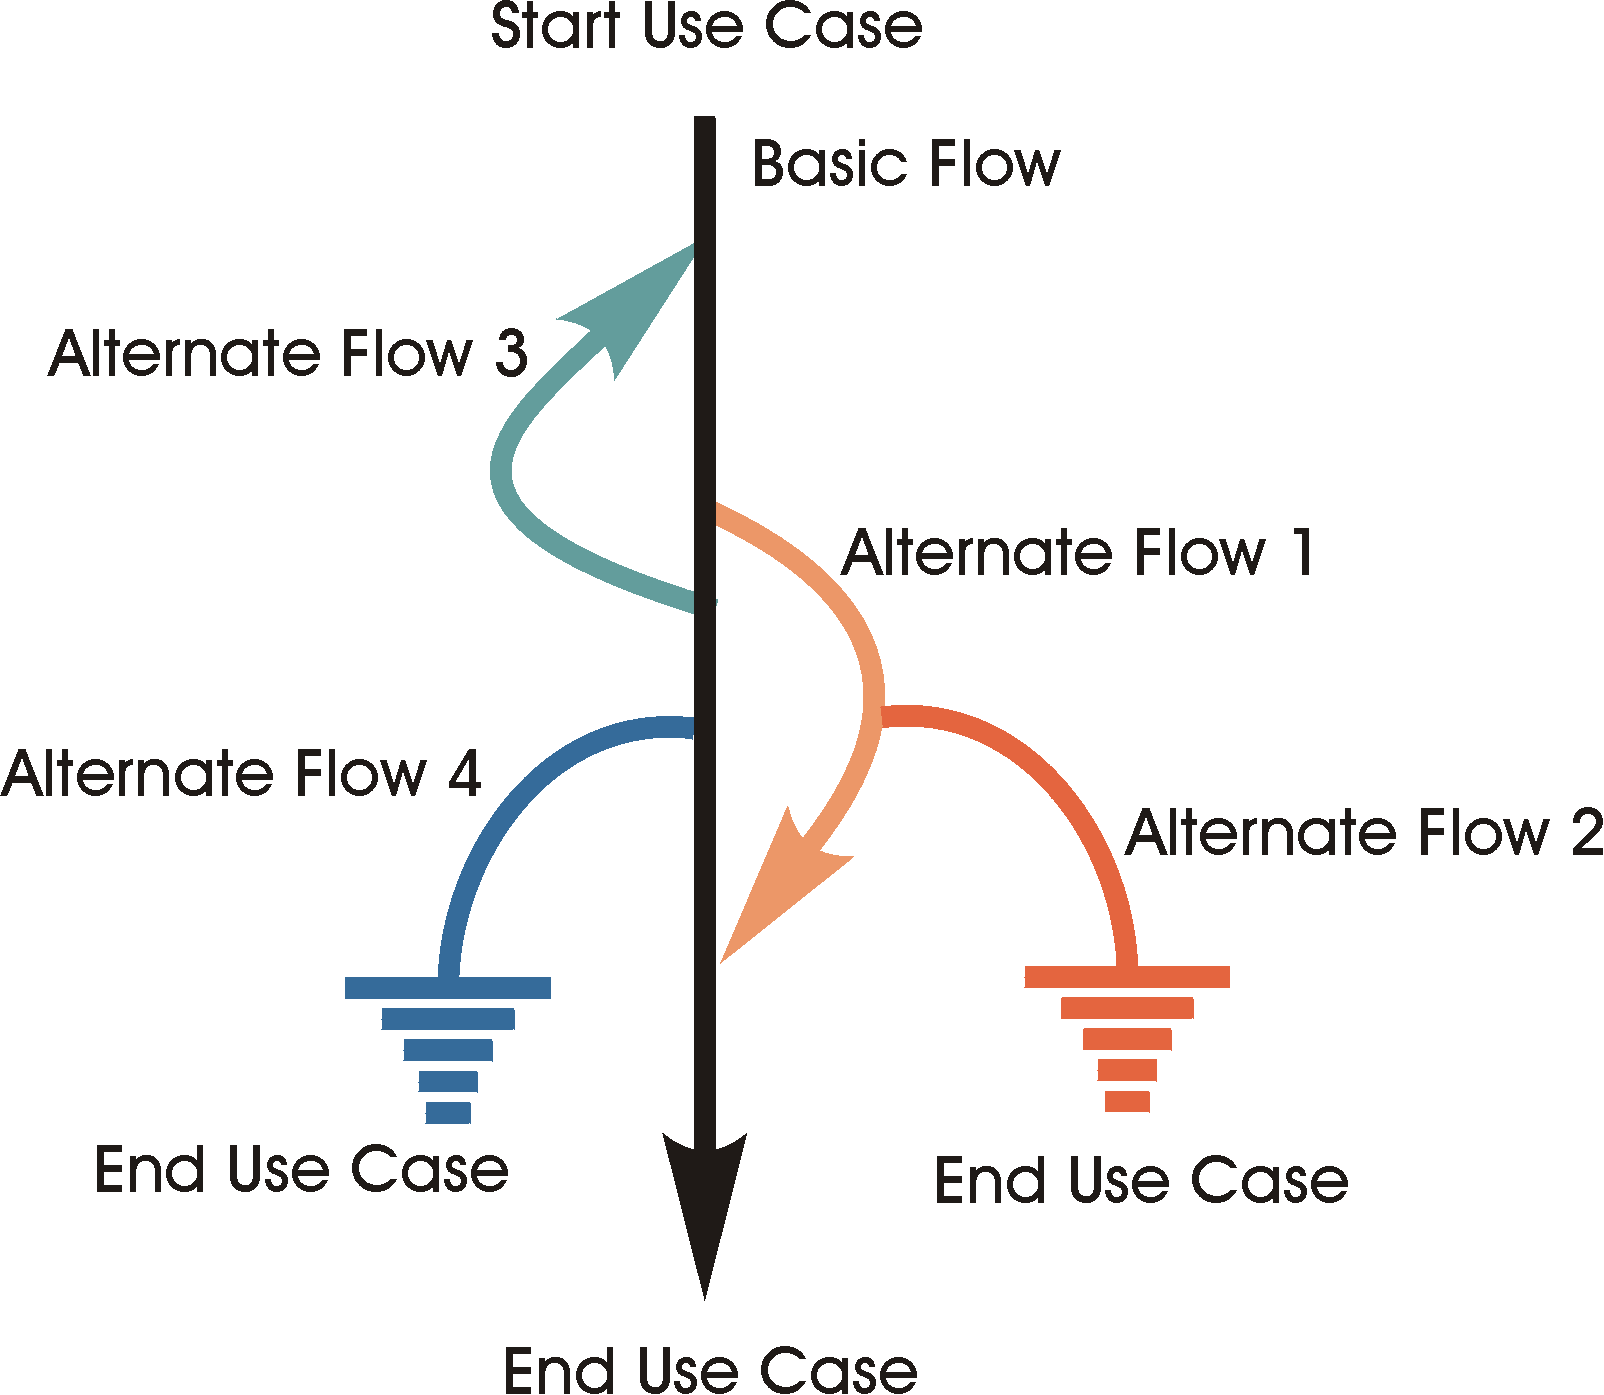
\includegraphics[scale=0.1]{02}\\  % o 0.9 indica 90% do tamanho original
{\small Fonte: Guideline: Test Case	- http://www.michael-richardson.com} %Fonte da imagem
\label{fig:exemplo} %rotulo para refencia
\end{figure}


\subsection{Seleção de Casos de Teste}
Como supracitado, a seleção desse subconjunto ou seleção de casos de teste, é praticada por seres humanos, e por consequência a tal, são suscetíveis a falhas humanas, em decorrência de diversos fatores como: Equívoca interpretação sobre requisitos extraídos de um documento de requisitos do software, relação entre experiencia técnica de tal testador para com formalidade da expressão de tais requisitos, elaboração erronia de tais requisitos no contato entre fornecedor e consumidor do produto, dentre outros.

Há de ressaltar que aplicação de testes de software não garante a corretude de um software ou algorítimo, onde como citado, necessita-se da aplicação de testes para todos os elementos pertencentes ao conjunto de possíveis entradas para o software, mas busca uma minimização de problemas ocasionais de tais falhas e uma maior segurança ao usuário final.

\subsection{Processamento de Línguas Naturais}
Essa área é responsável por compreender os mais variados aspectos e toda a estrutura gramatical de um idioma e a língua humana por meio de algorítimos para uma posterior abordagem das informações obtidas seja para reconhecimento e formulação de bases de conhecimento, automação de tarefas dependentes de avaliação ou interferência humana dentre outras inúmeras aplicações da tecnologia e ciência.
Com foco no presente projeto, discute-se o processamento textual de requisitos elicitados diretamente de um cliente como parte de um mercado consumidor e a abstração de informações com base em conhecimentos da Engenharia de Software para a construção de uma estrutura de um software e a seleção de casos de teste.

Para processar corpus textuais construídos em língua humana, é preciso reconhecer as estruturas gramaticais e sintáticas do respectivo idioma e processa-las segundo algum algorítimo de PLN que efetua avaliações probabilísticas sobre a sentença e sua composição para determinar classes gramaticais e aferir semanticamente qual o sentido do que está sendo compreendido, tudo isso atraves de arvores sintáticas como demonstrado a seguir:

\begin{figure}[!htb][H]
\centering
\caption{Árvore sintática da sentença em Inglês} %legenda
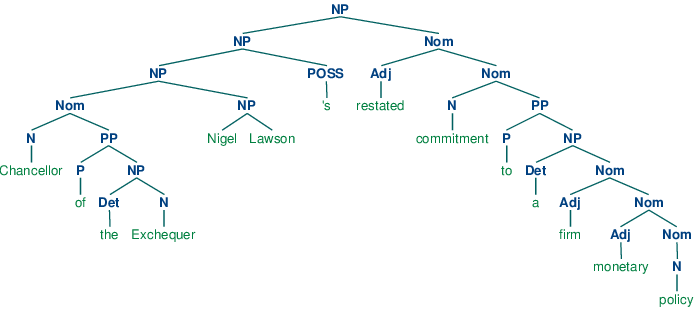
\includegraphics[scale=0.5]{01}\\  % o 0.9 indica 90% do tamanho original
{\small Fonte: Natural Language Toolkit - http://www.nltk.org} %Fonte da imagem
\label{fig:exemplo} %rotulo para refencia
\end{figure}

\section{Problema da Pesquisa}
Em países pertencentes ao polo de produção centralizada tecnológica, é amplo a gama de opções de ferramentas para auxiliar o papel do testador dentro das empresas, mas no cenário brasileiro, opções ainda são escassas. Essa escassez de ferramentas disponíveis para as empresas brasileiras de tecnologia da informação, reduzem a competitividade do país no setor bem como amplia os custos referente a cadeia de produção de softwares no Brasil.

A elevação dos custos supracitado, ainda pode decorrer em uma maior negligência por parte de tais corporações quanto a qualidade de sua produção, uma vez em que o alto custo empregado no processo de teste dos softwares pode não ser contemplado, aumentando assim, os riscos de insatisfação do mercado consumidor ou problemas em outras cadeias de produção, cujo é um componente agregado, o software em questão.

\section{Objetivo}
O objetivo da pesquisa do presente projeto busca avaliar de forma sistemática, a viabilidade da adoção para o idioma português de ferramentas de Processamento de Língua Natural existentes e desenvolvidas para o idioma Inglês, onde tangente a tal adoção, seja necessário mudanças pontuais nas estruturas de processamentos destes mecanismos para que seu funcionamento seja voltado para o idioma Português do Brasil.

Em futuras etapas de desenvolvimento do projeto, propõe-se a construção de uma ferramenta capaz de, a partir da entrada de um documento de requisitos e especificações de software, realizar a extração de informações necessárias para a construção e seleção de casos de teste, onde em seguida, seja capaz de gerar diagramas de sequencia, classe, dentre outros que beneficiem o processo de construção em modelo UML, a geração automatizada de maquinas de estado para que os testes extraídos e selecionados, possam ser executados de forma também automática, produzindo os resultados que auxiliaram o trabalho do testador e reduzirá a quantidade de falhas de software decorrentes de interferência humana, onde tal ferramenta para o idioma Português, ampliará a gama de opções disponíveis ao mercado brasileiro voltado para empresas de produção de software.

%%%%%%%%%%%%%%%%%%%%%%%%%%%%%%%%%%%%%%%%%%%%%%%%%%%%%%%%%%%%%
%O objetivo deste documento é apresentar o uso básico da classe {\tt uflamon} para a elaboração de monografias da UFLA utilizando a linguagem de marcação \LaTeX\ \cite{Lamport1994}.  A maioria dos comandos (macros) e ambientes das classes básicas da linguagem é válida também nessa classe, que é estendida com comandos para confecção da capa, páginas de rosto, dedicatórias, etc.

%A classe foi baseada inicialmente nas normas da PRPG/UFLA para produção de TCC \cite{PRPG2006}. Essas normas foram posteriormente atualidas, de maneira geral pela UFLA, para a produção de monografias, dissertações e teses \cite{BIB2010}.  A versão atual da {\tt uflamon} reflete a última versão da norma \cite{UFLA:2015}.

%Este texto, que objetiva apresentar um exemplo de uso da classe  {\tt uflamon}, encontra-se organizado como se segue. O Capítulo~\ref{cap:elementos} apresenta exemplos de inserção de figuras, tabelas, equações e demais elementos explicativos. O Capítulo~\ref{cap:conclusao} apresenta comentários e observações finais. Por fim, o Apêndice~\ref{cap:apendice} mostra como elaborar um apêndice simples.
\chapter{REFERENCIAL TEÓRICO}
\label{cap:referencial teórico}

O Processamento de Línguas Naturais possui grande enfoque nos dias atuais em decorrência da enorme gama de aplicações possíveis dentro das mais diversas áreas. Ramificado em alguns tipos, PLN possui técnicas e dificuldades especificas de cada diferente grupo. Destaca-se para o presente projeto, o processamento de textos em língua natural apresenta dificuldade em comuns com as outras áreas do PLN, como a omissão de informações, um problema cujo sua solução inexiste ou possui um tratamento extremamente complexo e limitado [CITAÇÃO ARTIGO UGMAR]; reconhecimento da variabilidade linguística onde podem existir termos ou construções sintáticas não reconhecidas pelas regras do processador em questão; ambiguidade em construções sintáticas que podem por sua vez levar a uma errônea classificação gramatical, reconhecimento de padrões de ironia tal que a interpretação semântica de um corpus completo ou uma única sentença possa ser equivocado; problemas clássicos e já conhecidos pelos pesquisadores e desenvolvedores da área de PLN a respeito de termos ou construções sintáticas complexas de se classificar mediante aplicação de um algorítimos (como uma característica de sua definição, sequencia lógica de instruções atômicas, livres de qualquer tipo de livre interpretação ou intuição. [CITAÇÃO: LIVRO DO SANDERSON PAA]).

O uso de PLN para extração de informações a partir de documentos de texto, eleva as taxas de sucesso quanto a interpretação das informações extraídos, onde uma vez aplicada em tarefas que dependem de um certo grau de interpretação arbitrária de um ser humano, é capaz de reduzir a quantidade de equívocos decorrentes de tal interferência.

A revisão da literatura executada ao decorrer da pesquisa, mostrou que o poder do processamento de línguas naturais podem alcançar resultados satisfatórios ao reconhecer requisitos de um projeto e interpreta-los, como demonstrado na publicação Automated Service Selection Using Natural Language Processing [REFERENCIA], onde a extração e a interpretação de 28 requisitos e 91 descrições de serviços em texto de um cliente consumidor, a partir de 15 serviços previamente selecionados por uma pessoa, obteve-se uma taxa de 53\% de acerto nos resultados. Tal resultado, demonstra que a aplicação de algorítimos mais robustos para a extração de informações podem possuir relevância para o auxilio a atividades humanas.

O livro Introdução ao Teste de Software [REFERENCIA] proveu a base para o estado da arte relacionado ao tema de teste de software, onde foca-se o objetivo principal do sistema a ser construído, a partir de um documento de requisitos, a extração de casos de teste, além disso, diversos outros documentos científicos foram revisados objetivando a obtenção do conhecimento a cerca do processamento de línguas naturais, seus desafios e métodos de implementação. Também foi preciso muito pesquisa em torno do campo de estudo relacionado a engenharia de software. Todos esses conhecimentos compõe o estado da arte do projeto.
\chapter{METODOLOGIAS E ANÁLISES}
\label{cap:metodologias e analises}

Ao decorrer do processo de pesquisa, foi executado uma revisão da literatura obtida através por chaves duplas {(Natural Language + Model Generation), (Natural Language + Test Model), (Requirement Document + Test Model), (Requirement Document + Information Extraction), (Requirement Document + Model Generation), (Natural Language + State Model), (Natural Language + State Machine), (Natural Language + Automation Test), (Natural Language + Automaton Generation)} onde foi coletado de diversas bases de dados, toda a literatura necessária para a fundamentação teórica do presente projeto bem como uma futura revisão sistemática para publicação.

Paralelamente a tal busca, um conjunto de ferramentas e bibliotecas conhecidas para processamento de línguas naturais (PLN) de código aberto, sob licença GNU/GPL - General Public License foram testadas objetivando o estudo do comportamento de seus algorítimos, taxas de sucesso/fracasso, informações de saída e entrada bem como suas implementações (neste caso avaliando possibilidades de alteração do código para o idioma português brasileiro, uma vez em que tais ferramentas trabalham com idioma Inglês, espanhol, dentre outros.).

\subsection{Stanford CoreNLP – Natural language software}
A primeira ferramenta a ser avaliada perante seu comportamento e sua estrutura estudada na pesquisa do presente projeto foi o parser de Stanford, CoreNLP. Aferiu-se que a ferramenta possui uma alta taxa de sucesso na estimativa das estruturas de um corpus de aproximadamente 98\% de sucesso. Esses altos índices de acerto deve-se ao fato de sua implementação interna atrelado ao uso de algorítimos para parsing como o poderoso parser Charniak, conforme verificou-se em estudos de sua estrutura de core.

\begin{figure}[H]
\centering
\caption{Implementações do software CoreNLP} %legenda
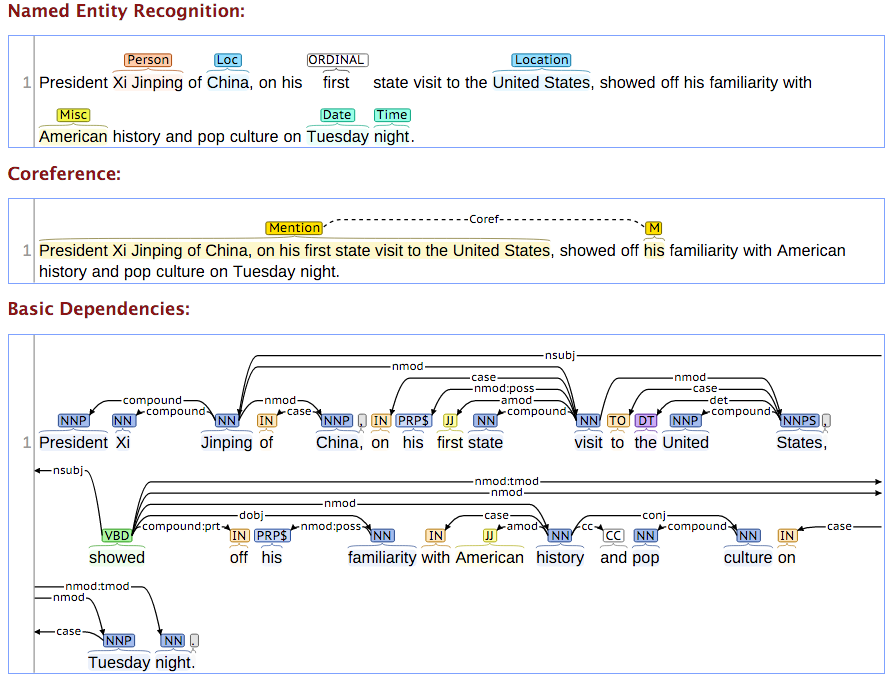
\includegraphics[scale=0.4]{03}\\  % o 0.9 indica 90% do tamanho original
{\small Fonte: Stanford CoreNLP - https://stanfordnlp.github.io} %Fonte da imagem
\label{fig:exemplo} %rotulo para refencia
\end{figure}

Em um primeiro momento, a presente ferramenta foi o principal candidato para a incorporação no sistema proposto no projeto, viável, uma vez em que possui licença GNU/GPL - General Public License e código aberto. Seria necessário desenvolver e adicionar um módulo para o processamento de língua no idioma Português, haja visto que a ferramenta implementa o seguinte conjunto de idiomas: Árabe, Inglês. Espanhol, Alemão, Frances e Chines. Os resultados de tal escolha e modificação serão discutidos posteriormente na seção de de Resultados deste documento.

\subsection{Poli-Libras}
Uma ferramenta de tradução automática de textos escritos em idioma português para sequencia de sinais de Libras (Linguagem Brasileira de Sinais) por meio de interface gráfica e vetores que representam uma personagem humana reproduzindo os sinais traduzidos. O poli-libras conta com diversos módulos, onde demonstra-se viável o reaproveitamento e a incorporação (haja visto que ambos o projeto possui licença GNU/GPL - General Public License) ao projeto apresentado por via do presente documento.

Um módulo encontrado na implementação do Poli-Libras é útil: Módulo de geração da árvore sintática responsável pelo processo de parsing de um determinado corpus redigido em idioma Português brasileiro.

\begin{figure}[H]
\centering
\caption{Projeto arquitetural do software Poli-Libras} %legenda
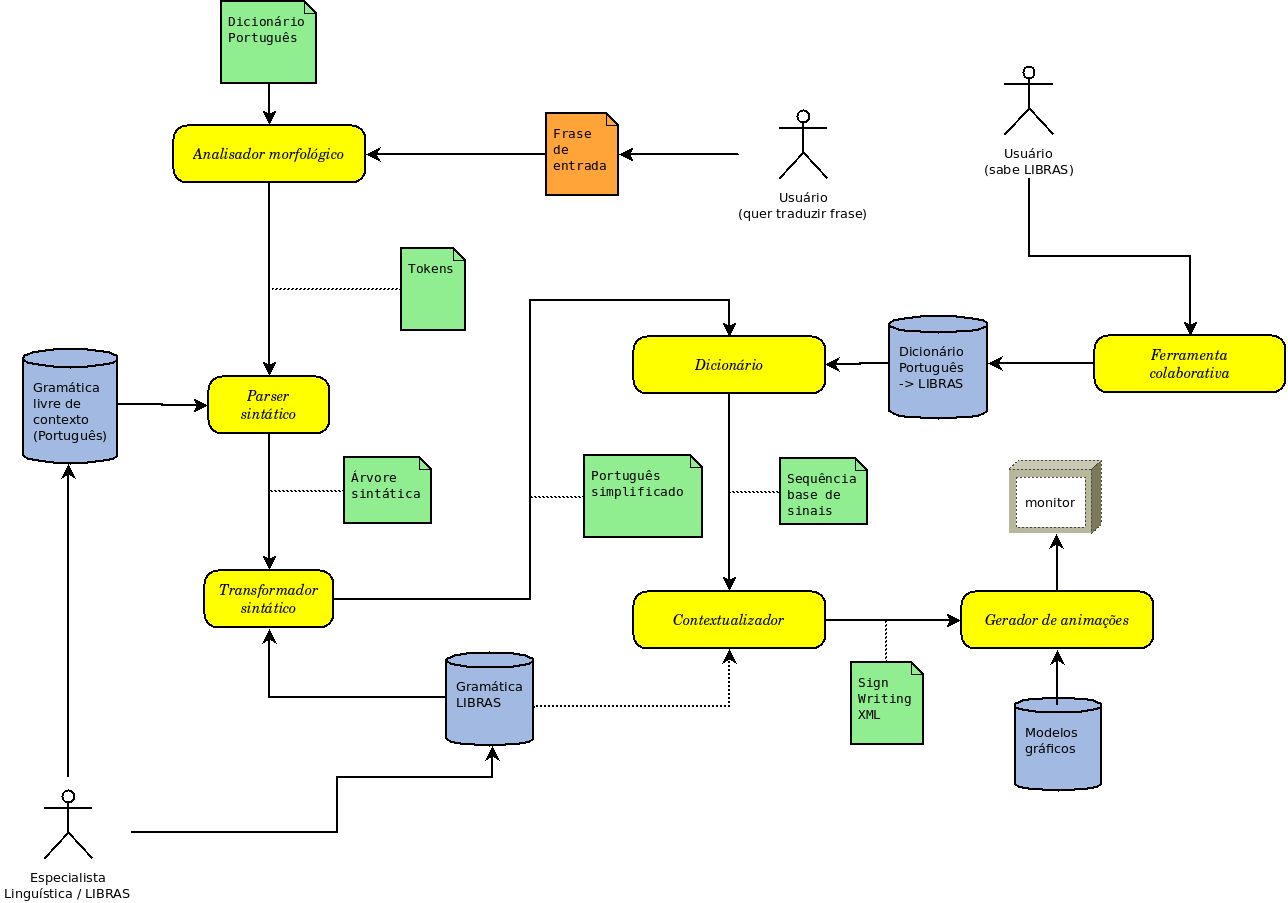
\includegraphics[scale=0.325]{arquitetura}\\  % o 0.9 indica 90% do tamanho original
{\small Fonte: Poli-Libras - http://www.polilibras.com.br/desenvolvimento/tradutor} %Fonte da imagem
\label{fig:exemplo} %rotulo para refencia
\end{figure}

\subsection{NILC's Taggers}
Uma ferramenta tagger utilizada para mapear um corpus textual, classificando todos os termos que o compõem em classes gramaticais, que posteriormente, poderão ser analisados pelo módulo de parsing do projeto para se obter a árvore sintática e assim, tornar possível a extração de informações com base em construções gramaticais conhecidas.

Essa ferramenta trabalha com um padrão internacional e pré estabelecido para definições das tags (tagset), denominado MXPOST, onde a implicação deste fato, será posteriormente abordado no presente documento.


\subsection{CoGrOO - Corretor Gramatical}
A descoberta da ferramenta CoGrOO será abordada posteriormente no presente documento. CoGrOO é uma ferramenta desenvolvida para a suíte de ferramentas Libre Office, de licença livre GNU/GPL - General Public License Version 3.0 e open source, responsável pela analise de corpus textuais objetivando a identificação de erros gramaticais segundo o idioma Português brasileiro.

A ferramenta demonstra-se poderosa e capaz de detectar os seguintes erros gramaticais: colocação pronominal; concordância nominal; concordância entre sujeito e verbo; concordância verbal; uso de crase; regência; nominal; regência verbal.

\subsection{Análise}
Todas as ferramentas supracitadas foram analisadas quanto ao nível de input e output, objetivando se as saídas produzidas cobrem as necessidades do vingante projeto como por exemplo a construção da árvore sintática, a classificação das estruturas gramaticais, um corpus pré processado por um tagger, dentre outros aspectos.
Ao decorrer da presente fase de desenvolvimento da pesquisa, estudou-se toda a estrutura e arquitetura das ferramentas analisadas, possibilitado pela natureza open source.
\chapter{RESULTADOS}
\label{cap:resultados}

Os resultados obtidos com a presente etapa da pesquisa são de enorme relevância para a futura implementação do projeto, pois determinados aspectos observados, modificaram a decisão a ser tomada quanto a ferramenta que será posteriormente incorporada ao projeto vigente.

A principal ferramenta candidata quanto a incorporação até o momento era CoreNLP, processador de língua natural de Stanford University, uma vez em que tal ferramenta possui uma completa e robusta estrutura para construção das árvores sintáticas bem como quanto a geração de informações necessárias para o sistema a ser trabalhado. Ao detalhar-se o código e a estrutura do CoreNLP, denotou-se que seria necessário a adição e construção de um módulo independente para o idioma português, seguindo a estruturação dos módulos de Árabe, Espanhol, Chinês, Alemão e Francês.

Conforme as execuções, a ferramenta necessita de um corpus textual em um dos determinados idiomas previamente conhecidos pelo CoreNLP e parâmetros para a definição do idioma e métodos de analises a serem utilizados.

\begin{figure}[H]
\centering
\caption{Executando CoreNLP sobre um corpus textual} %legenda
\begin{Verbatim}[fontsize=\small]
$ echo "the quick brown fox jumped over the lazy dog" > input.txt
$ java -mx3g edu.stanford.nlp.pipeline.StanfordCoreNLP -outputFormat json -file input.txt
\end{Verbatim} 
{\small Fonte: Teste executado.} %Fonte da imagem
\label{fig:exemploconfig} %rotulo para refencia
\end{figure}

\begin{figure}[H]
\centering
\caption{Saída CoreNLP sobre um corpus textual} %legenda
\begin{Verbatim}[fontsize=\small]
$ echo "the quick brown fox jumped over the lazy dog" > input.txt
$ java -mx3g edu.stanford.nlp.pipeline.StanfordCoreNLP -outputFormat json -file input.txt
\end{Verbatim} 
{\small Fonte: Teste executado.} %Fonte da imagem
\label{fig:exemploconfig} %rotulo para refencia
\end{figure}

Ao decorrer do estudo sobre a arquitetura da ferramenta, denotou-se que haveria de ser desenvolvido um módulo para o idioma Português brasileiro, no entanto, todos os módulos de todos os idiomas previamente desenvolvidos, usufruem da ferramenta Cogroo, com exceção do idioma Inglês nativo.

Em sua complexa estrutura, a ferramenta conta com um objeto responsável por efetuar o mapeamento do corpus fornecido ao sistema para com os objetivos do usuário, seja aplicar o mecanismo de tagger ou executar uma analise morfossintática sobre cada sentença de entrada.

\begin{figure}[H]
\centering
\caption{Objeto de mapeamento do sistema} %legenda
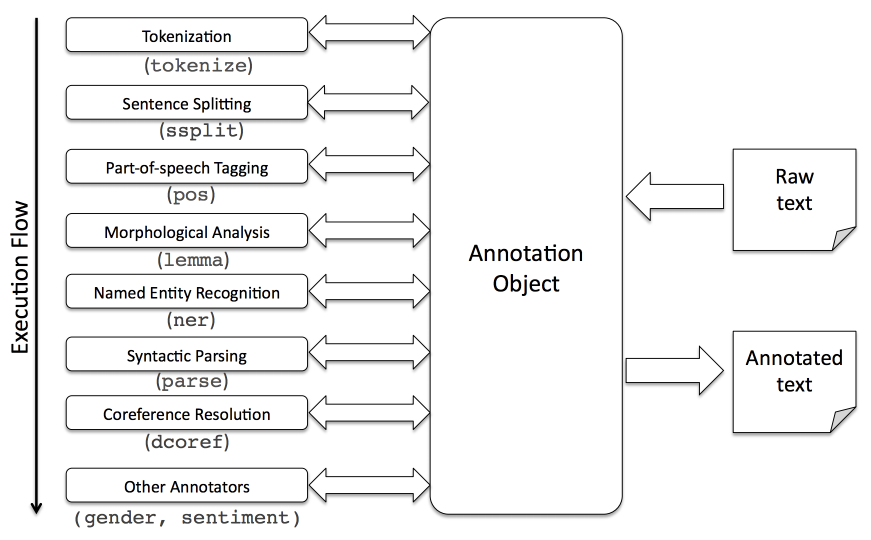
\includegraphics[scale=0.4]{AnnotationPipeline}\\  % o 0.9 indica 90% do tamanho original
{\small Fonte: CoreNLP Community - stanfordnlp.github.io} %Fonte da imagem
\label{fig:exemplo} %rotulo para refencia
\end{figure}

Este mecanismo auxiliaria a integração com o sistema a ser desenvolvido no presente projeto, uma vez em que somente específicas informações e não todas que o CoreNLP oferece seriam necessárias para que fosse possível a extração da informação a partir de um documento de requisitos de entrada.

\begin{figure}[H]
\centering
\caption{Exemplo de invocação dos módulos} %legenda
\begin{lstlisting}
public AnnotationPipeline buildPipeline() {
    AnnotationPipeline pl = new AnnotationPipeline();
    pl.addAnnotator(new TokenizerAnnotator(false));
    pl.addAnnotator(new WordsToSentencesAnnotator(false));
    pl.addAnnotator(new POSTaggerAnnotator(false));
    pl.addAnnotator(new MorphaAnnotator(false));
    pl.addAnnotator(new TimeAnnotator("sutime", props));
    pl.addAnnotator(new PhraseAnnotator(phrasesFile, false));
    return pl;
}
\end{lstlisting} 
{\small Fonte: CoreNLP Community - stanfordnlp.github.io} %Fonte da imagem
\label{fig:exemplocodigo1} %rotulo para refencia
\end{figure}


Segundo os parâmetros passados ou em uma possível integração com outro sistema, por via de APIs, as propriedades configuradas e os métodos invocados através do objeto mapeador, a ferramenta é capaz de gerar as seguintes saídas:

\begin{figure}[H]
\centering
\caption{Trechos de Discurso} %legenda
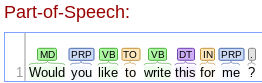
\includegraphics[scale=0.9]{01a}\\  % o 0.9 indica 90% do tamanho original
{\small Fonte: Execução da Ferramenta} %Fonte da imagem
\label{fig:exemplo} %rotulo para refencia
\end{figure}

\begin{figure}[H]
\centering
\caption{Lemas} %legenda
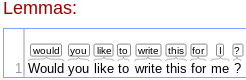
\includegraphics[scale=0.9]{02b}\\  % o 0.9 indica 90% do tamanho original
{\small Fonte: Execução da Ferramenta} %Fonte da imagem
\label{fig:exemplo} %rotulo para refencia
\end{figure}

\begin{figure}[H]
\centering
\caption{Reconhecimento de Entidades} %legenda
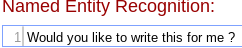
\includegraphics[scale=0.9]{03c}\\  % o 0.9 indica 90% do tamanho original
{\small Fonte: Execução da Ferramenta} %Fonte da imagem
\label{fig:exemplo} %rotulo para refencia
\end{figure}

\begin{figure}[H]
\centering
\caption{Árvore Sintática} %legenda
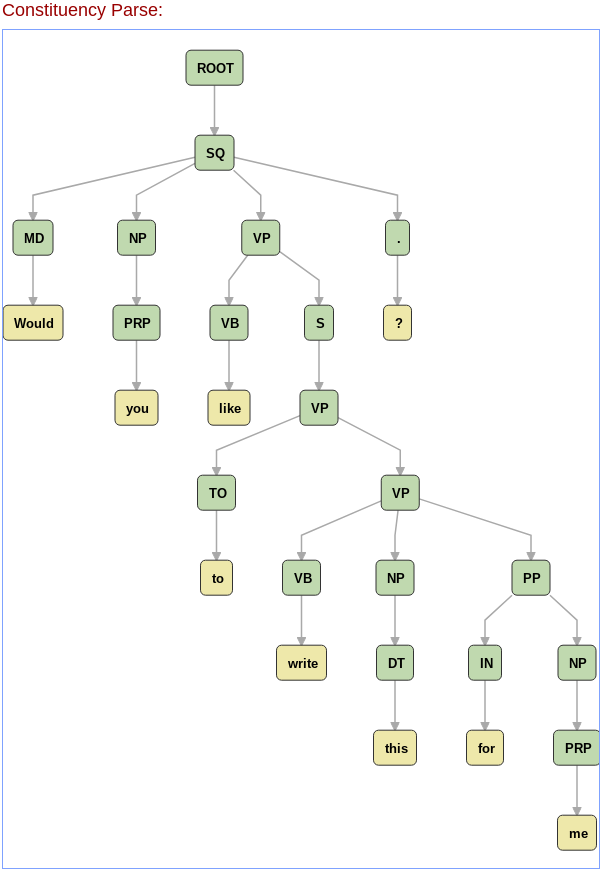
\includegraphics[scale=0.6]{04d}\\  % o 0.9 indica 90% do tamanho original
{\small Fonte: Execução da Ferramenta} %Fonte da imagem
\label{fig:exemplo} %rotulo para refencia
\end{figure}

\begin{figure}[H]
\centering
\caption{Árvore de Dependências} %legenda
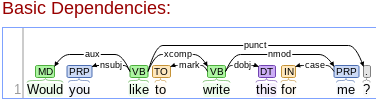
\includegraphics[scale=0.9]{05e}\\  % o 0.9 indica 90% do tamanho original
{\small Fonte: Execução da Ferramenta} %Fonte da imagem
\label{fig:exemplo} %rotulo para refencia
\end{figure}

\begin{figure}[H]
\centering
\caption{Árvore de Dependências} %legenda
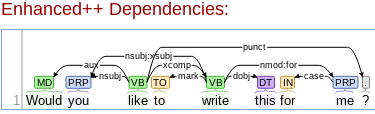
\includegraphics[scale=0.9]{06f}\\  % o 0.9 indica 90% do tamanho original
{\small Fonte: Execução da Ferramenta} %Fonte da imagem
\label{fig:exemplo} %rotulo para refencia
\end{figure}

\begin{figure}[H]
\centering
\caption{IE} %legenda
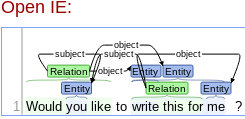
\includegraphics[scale=0.9]{07g}\\  % o 0.9 indica 90% do tamanho original
{\small Fonte: Execução da Ferramenta} %Fonte da imagem
\label{fig:exemplo} %rotulo para refencia
\end{figure}

\begin{figure}[H]
\centering
\caption{Conferência} %legenda
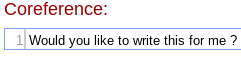
\includegraphics[scale=0.9]{08h}\\  % o 0.9 indica 90% do tamanho original
{\small Fonte: Execução da Ferramenta} %Fonte da imagem
\label{fig:exemplo} %rotulo para refencia
\end{figure}

\begin{figure}[H]
\centering
\caption{Relações KBP} %legenda
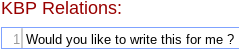
\includegraphics[scale=0.9]{10j}\\  % o 0.9 indica 90% do tamanho original
{\small Fonte: Execução da Ferramenta} %Fonte da imagem
\label{fig:exemplo} %rotulo para refencia
\end{figure}

\begin{figure}[H]
\centering
\caption{Análise de Sentimento} %legenda
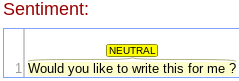
\includegraphics[scale=0.9]{11j}\\  % o 0.9 indica 90% do tamanho original
{\small Fonte: Execução da Ferramenta} %Fonte da imagem
\label{fig:exemplo} %rotulo para refencia
\end{figure}

Outra ferramenta avaliada, Poli-Libras, um sistema de tradução de um corpus textual para Língua Brasileira de Sinais (LIBRAS) intermediado por uma interface gráfica, demonstra-se relevante para o presente projeto, uma vez em que é composta por mecanismos de analise sintática para o idioma português brasileiro, para o qual acarreta grande vantagem em facilitar de desenvolvimento do sistema em questão.

Não existe maneira de se executar o Poli-Libras somente com simples entrada e saída objetivando somente a analise das informações e construções do software como a ferramenta anteriormente discutida, uma vez em que ela foca diretamente na integração com outro sistema através de módulos ou eu seu próprio sistema nativo, com a interface gráfica e outros módulos satélites.

A ferramenta Tagger desenvolvida núcleo NILC, também foi alvo dos estudos na presente etapa do projeto. Caso a opção de ferramenta escolhida fosse o Poli-Libras, haveria necessidade de utilizarmos uma ferramenta do tipo tagger para mapear todo um corpus textual de entrada, no caso, um documento de requisitos, para que fosse possível o parsing e a extração das informações necessárias.

\begin{figure}[H]
\centering
\caption{Exemplo de corpus textual mapeado com o tagger desenvolvido pelo NILC} %legenda
\begin{Verbatim}[fontsize=\small]
._.
Surgiu_VINT ,_, então_ADV ,_, a_ART atualmente_ADV aceita_ADJ 
teoria_N da_PREP+ART biogênese_N ._.
Teoria_N da_PREP+ART abiogênese_N :_: os_ART seres_N vivos_ADJ
originam-se_VBI+PPOA da_PREP+ART matéria_N bruta_ADJ de_PREP 
maneira_N contínua_ADJ ._.
Teoria_N da_PREP+ART biogênese_N :_: os_ART seres_N vivos_ADJ 
originam-se_VBI+PPOA de_PREP outros_ADJ seres_N vivos_ADJ ._.
Von_NP Helmont_NP (_( 1600_NC )_) ,_, o_ART maior_ADJ 
fisiologista_N da_PREP+ART época_N ,_, dá_VTD várias_ADJ 
receitas_N para_PREP a_ART abiogênese_N ._. Uma_ART delas_PREP+PPR
é_VLIG a_ART fórmula_N para_PREP se_PAPASS obter_VTD ratos_N :_: 
"_" enche-se_VBI+PPOA de_PREP trigo_N e_CONJCOORD fermento_N 
um_ART vaso_N ,_, que_PR é_VAUX fechado_VTD com_PREP uma_ART 
camisa_N suja_ADJ ,_, de_PREP preferência_N de_PREP mulher_N ._.
\end{Verbatim} 
{\small Fonte: NILC Website.} %Fonte da imagem
\label{fig:exemploconfig} %rotulo para refencia
\end{figure}

Os conjuntos de tags definidos por padrões internacionais de tagset possibilitam a integração entre a ferramenta de tagger e a ferramenta de processamento de língua natural. Caso a opção escolhida fosse a ferramenta CoreNLP, não haveria necessidade do uso de um tag, haja visto que existem módulos em sua robusta construção, que promovem o mapeamento por meio das tags de um corpus textual de entrada.

Concluindo a presente etapa de pesquisa, analisou-se a ferramenta Cogroo, o corretor gramatical livre e open source da suíte de aplicativos Libre Office. Esta ferramenta destacou-se por estar presente em todas as demais ferramentas supracitadas, exceto Poli-Libras e Nilc Tagger, atraindo o foco para ser a atual e mais provável candidata a incorporação ao sistema. Uma ferramenta robusta, com elevada taxa de acerto na classificação gramatical, possui API de integração com outros sistemas, irá facilitar amplamente o desenvolvimento do projeto em questão.

Cogroo é capaz de prover algumas informações de saída quando recebe um corpus textual como entrada, onde a estrutura resultante mais importante e necessária é a árvore sintática, de onde pode-se extrair os dados relevantes para classificação das estruturas gramaticais presentes no corpus e assim possibilitar a averiguação de estruturas conhecidas como casos de teste, entidades do sistema, dentre outros.

\begin{quadro}[H]
  \begin{center}
    \caption{Exemplo de execução da ferramenta sobre a sentença: "O futuro está em processamento de línguas naturais."} 
    \label{tab:exemplo}
    \vspace{0.1cm}
    \footnotesize
    \begin{tabular}{|c|c|c|c|c|c|c|}
      \hline
      N# & Elemento & Lemas & Classe & Flexão & Sintagma & Função \\
      \hline
      \hline
      1 & O & o & artigo & masculino, singular & nominal & sujeito\\
      2 & futuro & futuro & substantivo & masculino, singular & nominal & sujeito\\
      3 & está & estar & verbo infinitivo & presente, terceira pessoa, singular, indicativo & verbal & predicado\\
      4 & em & em & preposição & - & preposicional & complemento adverbial\\
      5 & processamento & processamento, processar & substantivo & masculino, singular & nominal & complemento adverbial\\
      6 & de & de & preposição & - & preposicional & complemento adverbial\\
      7 & línguas & língua & substantivo & feminino, plural & nominal & complemento adverbial\\
      8 & naturais & natural & adjetivo & feminino, plural & nominal & complemento adverbial\\
      \hline 
    \end{tabular}
  \end{center}
  \centering {\small Fonte: Saída da execução} %Fonte do quadro
\end{quadro}

\begin{figure}[H]
\centering
\caption{Árvore sintática gerada pela ferramenta Cogroo} %legenda
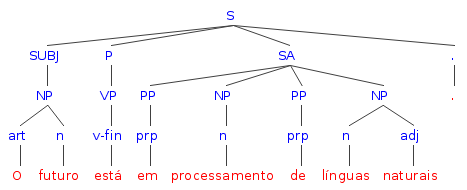
\includegraphics[scale=0.6]{stgraph}\\  % o 0.9 indica 90% do tamanho original
{\small Fonte: Execução da Ferramenta} %Fonte da imagem
\label{fig:exemplo} %rotulo para refencia
\end{figure}

Além do teste e estudo das estruturas e arquiteturas das ferramentas em questão, foi executado uma revisão bibliográfica da literatura objetivando a identificação dos principais métodos para a extração da informação através de documentos textuais, inclusive com trabalhos que especificam documentos de requisitos para empresas de tecnologia da informação. Denotou-se também os principais desafios da aplicação dos métodos de extração de informações com base em problemas já conhecidos do campo de pesquisa em processamento de línguas naturais.

Sabe-se que os principais problemas no tratamento de PLN para o presente projeto enquadra-se em ambiguidade de sentenças, omissão de informação por parte do redator do corpus textual e construções gramaticais não suportadas pela ferramenta de PLN a ser utilizada. Para algum desses desafios, certos autores apresentam soluções como verificado na construção da ferramenta UGMAR [REFERENCIA DO ARTIGO] onde o autor propõe soluções para desambiguação de sentenças, reconstrução de certas informações omitidas, claro que com um nível muito restrito de limitação e arquiteturas para o desenvolvimento destes mecanismos.
\chapter{CONCLUSÃO}
\label{cap:conclusao}

Como supracitado na sessão de introdução do presente documento, essa etapa de pesquisa foi de enorme relevância para a decisão a respeito da viabilidade da aplicação de uma ferramenta de processamento de língua natural já existente sobre o projeto do sistema. Foram estudadas e testadas ferramentas que trabalham com o idioma Português brasileiro e Inglês, onde estas objetivaram o aproveitamento de seus mecanismos internos, onde talvez fossem necessário, como constatado nos capítulos anteriores, somente algumas alterações para integração com o sistema e construção dos módulos de suporte para o idioma Português.

Ao decorrer da pesquisa, foi adicionado a gama de possíveis ferramentas, o corretor gramatical Cogroo, desenvolvido para a suíte de aplicativos Libre Office e mantido sobre licença GNU/GPL - General Public License e código aberto. Cogroo deste então, devido a facilidade de integração com o sistema e sua robustez para com o tratamento de sentenças em língua natural sobre o idioma Português brasileiro, tornou-se o principal e escolhido candidato a ser implantado no sistema para a função de processamento da língua natural, fornecendo informações relevantes para a etapa posterior de extração da informação, com base na identificação das estruturas gramaticais.

A partir dos estudos sobre o core do código da ferramenta CoreNLP, principal candidata antes do Cogroo, constatou-se de que haverá necessidade da implementação de um módulo para analise do idioma Português brasileiro, contribuindo assim inclusive com o a evolução da ferramenta através da comunidade.

A partir da revisão bibliográfica da literatura que trata a respeito dos temas de processamento de línguas naturais e extração da informação, abstraiu-se a viabilidade de se desenvolver o presente sistema, extraindo relevantes informações a partir de um documento de requisitos e classificando com o fim de se identificar entidades, estruturas e casos de teste de um projeto de software. Verificou-se também os desafios dessa construções, em que tangem problemas relacionados ao processamento de línguas naturais e possíveis soluções para o mesmo.

Será necessário propor um modelo padronizado rigidamente de documentação de requisitos de software bem como avaliação das taxas de acerto da ferramenta candidata escolhida para corpus textuais do conteúdo relacionado ao que será fornecido para o programa.

Toda tal revisão da literatura foi crucial para o desenvolvimento dos conhecimentos na área de processamento de línguas naturais, teste de software e engenharia de software, todo o estado da arte que compõe o projeto e a conjunção de todas essas áreas de estudo.
%\chapter{ELEMENTOS DO TEXTO}
\label{cap:elementos}

Este capítulo apresenta o uso básico de equações, figuras e tabelas no código da monografia, bem como o posicionamento das legendas, segundo as normas da UFLA.

\section{Utilizando Recursos do \LaTeX}

\subsection{Inserindo Comandos Definidos}

Esta subseção apresenta o uso de comandos definidos pelo usuário no preâmbulo do arquivo principal \LaTeX e alguns exemplos do modo matemático. Por exemplo, na texto a seguir é utilizado o comando  \verb+\defs+, definido anteriormente pelo próprio autor do texto:

\begin{quote}
Os conjuntos fundamentais da teoria são os \defs{conjuntos elementares}. Se $E$ é um conjunto elementar, $des(E)$ denota a descrição dessa classe de equivalência. Essa descrição é função do conjunto de atributos que define $R$. Note que, dados $x,y \in E$, onde $E$ é um conjunto elementar em $A$, $x$ e $y$ são indiscerníveis, i.e., no espaço $A=(U,R)$ não se consegue distinguir $x$ de $y$, pois $des(x) = des(y) = des(E)$. 
\end{quote}

\subsection{Inserindo Figuras}

A Figura~\ref{fig:exemplo} é apenas um exemplo de figura para que o usuário da classe possa saber como uma figura pode ser inserida e referenciada automaticamente no texto.É importante observar que legendas de figuras ficam abaixo de seu conteúdo.

\begin{figure}[!htb]
\centering
\caption{Uma Figura de Exemplo} %legenda

\includegraphics[scale=0.9]{gradpenguin}\\  % o 0.9 indica 90% do tamanho original
% pdfLaTeX aceita figuras no formato PNG, JPG ou PDF
% figuras vetoriais podem ser exportadas para eps e depois convertidas para pdf usando epstopdf
{\small Fonte: fonte da figura} %Fonte da imagem
\label{fig:exemplo} %rotulo para refencia
\end{figure}

\subsection{Inserindo Saídas de Comandos e Código}

A menos que sejam trechos pequenos, saídas de comandos, trechos de arquivos de configuração e código de aplicativos devem ser inseridos como figura, como mostrado, respectivamente, na Figura~\ref{fig:exemplocomando}, Figura~\ref{fig:exemploconfig} e Figura~\ref{fig:exemplocodigo1}. Para comandos e configuração, recomenda-se o uso do pacote {\tt fancyvrb}, o que pode ser visto na Figura~\ref{fig:exemplocomando} e Figura~\ref{fig:exemploconfig}.

Para inserção de código, recomenda-se o uso do pacote {\tt listings}, que permite melhor apresentação do mesmo, o que é mostrado na Figura~\ref{fig:exemplocodigo1}. Além disso, esses dois pacotes permitem a inserção de texto/código em arquivos externos, sem inclusão direta no arquivo \LaTeX. Isso pode ser verificado no exemplo de uso do {\tt listings} apresentado na Figura~\ref{fig:exemplocodigo2}

\begin{figure}[!htb]
\centering
\caption{Inserindo Comando} %legenda
\begin{Verbatim}[fontsize=\small]
$ dir monografia*
-rw-r--r--  1 joukim users   3650 Set 12 17:56 monografia.aux
-rw-r--r--  1 joukim users   6366 Set 12 17:43 monografia.bbl
-rw-r--r--  1 joukim users    290 Set 12 17:56 monografia.lof
-rw-r--r--  1 joukim users  27937 Set 12 17:56 monografia.log
-rw-r--r--  1 joukim users    194 Set 12 17:56 monografia.lot
-rw-r--r--  1 joukim users    715 Set 12 17:56 monografia.out
-rw-r--r--  1 joukim users 159243 Set 12 17:56 monografia.pdf
-rw-r--r--  1 joukim users   4559 Set 12 17:47 monografia.tex
-rw-r--r--  1 joukim users    964 Set 12 17:56 monografia.toc
\end{Verbatim} 
%$ - esse comentário é para não confundir editor de texto
{\small Fonte: fonte da figura} %Fonte da imagem
\label{fig:exemplocomando} %rotulo para refencia
\end{figure}

\begin{figure}[!htb]
\centering
\caption{Inserindo Trecho de Arquivo de Configuração} %legenda
\begin{Verbatim}[fontsize=\small]
// named.conf for Red Hat caching-nameserver
options {
        directory "/var/named";
        dump-file "/var/named/data/cache_dump.db";
        statistics-file "/var/named/data/named_stats.txt";
        // query-source address * port 53;
};
\end{Verbatim} 
{\small Fonte: fonte da figura} %Fonte da imagem
\label{fig:exemploconfig} %rotulo para refencia
\end{figure}


\begin{figure}[!htb]
\centering
\caption{Inserindo Código Diretamente no Arquivo \LaTeX} %legenda
\begin{lstlisting}
// exit the program
public void on_buttonExit_clicked() {
	System.exit(0);
}

// copy data
public void on_buttonCopy_clicked() {
	labelShow.setText(entryData.getText());
}

// print version of Java
public static void main(String[] args) {
	System.out.println(System.getProperty("java.fullversion"));
}
\end{lstlisting} 
{\small Fonte: fonte da figura} %Fonte da imagem
\label{fig:exemplocodigo1} %rotulo para refencia
\end{figure}


\begin{figure}[H]
\centering
\caption{Inserindo Código a Partir do Código-Fonte} %legenda
\label{fig:exemplocodigo2} %rotulo para refencia
\lstinputlisting{Hello.java}
{\small Fonte: fonte da figura} %Fonte da imagem
\end{figure}

\subsection{Inserindo Quadros e Tabelas}

Escrever um quadro ou tabela e referenciá-los é bem simples. Por exemplo o Quadro~\ref{tab:exemplo} ilustra a criação de um quadro, tendo aqui seu referenciamento no texto. É importante observar o posicionamento da legenda antes do corpo da tabela e da fonte após. Outros exemplos são mostrados na Tabela~\ref{tab:outro} e Tabela~\ref{tab:maisum}.

\begin{quadro}[htb]
  \begin{center}
    \caption{Exemplo de Quadro} 
    \label{tab:exemplo}
    \vspace{0.2cm}
    \footnotesize
    \begin{tabular}{|c|c|c|c|c|c|}
      \hline
      $U$ & $vitA$ & $vitC$ & $vitD$ & $prot$ & $lip$ \\
      \hline
      \hline
      $d_1$ & 1 & 3 & 4 & 2 & 3\\
      $d_2$ & 1 & 3 & 3 & 3 & 2\\
      $d_3$ & 1 & 3 & 4 & 3 & 1\\
      $d_4$ & 3 & 5 & 2 & 5 & 2\\
      $d_5$ & 4 & 5 & 2 & 5 & 1\\
      $d_6$ & 3 & 5 & 2 & 3 & 4\\
      $d_7$ & 4 & 4 & 1 & 3 & 2\\
      \hline 
    \end{tabular}
  \end{center}
  \centering {\small Fonte: fonte do quadro} %Fonte do quadro
\end{quadro}

\begin{table}[!htb]
\begin{center}
  \caption{Recursos do {\ttfamily syslog}}
  \label{tab:outro}
  \small
  \begin{tabular}{l|p{9cm}}
    \hline
    \rowcolor[gray]{.9}
    \bf Recurso & \bf {\em Daemons} Associados (Alguns Exemplos) \\
    \hline
    \hline
    \tt kern & \em kernel  \\
    \tt user & processos dos usuários ({\tt ntpd}) \\
    \tt mail & softwares relacionados com o correio eletrônico ({\tt sendmail})\\
    \tt daemon & {\em daemons} do sistema ({\tt gated}, {\tt inetd}, 
    {\tt named}, {\tt ntpd})\\
    \tt auth &  comandos relacionados à autorização e segurança 
    ({\tt login}, {\tt rlogin}, {\tt su}, {\tt passwd}) \\
    \tt lpr & spool de impressão ({\tt lpd})\\
    \tt news & sistema de notícias da usenet ({\tt nnrpd})\\
    \tt uucp & destinado ao {\tt uucp}\\
    \tt cron & relacionado ao {\em daemon} {\tt cron}\\
    \tt mark &  registros de data/hora gerados a intervalos regulares 
    ({\tt syslogd})\\
    \tt local0-7 & 8 tipos de mensagens locais \newline
    ({\tt tcpd -- local7}, {\tt sudo -- local2}, {\tt popper - local0}) \\
    \tt syslog &  mensagens internas ao {\tt syslog}\\
    \tt authpriv & mensagens privadas de autorização\\
    \tt ftp & associado ao {\tt ftpd} ({\em daemon} do {\tt ftp}) \\
    \tt * &  todos os recursos com exceção do {\tt mark}\\
    \hline
  \end{tabular}
\end{center}
\centering {\small Fonte: fonte da tabela} %Fonte da tabela
\end{table}

\begin{table}[!htb]
\caption{Opções do Comando {\ttfamily at}}
\label{tab:maisum}
\begin{center}
  \small
  \begin{tabular}{l|p{9cm}}
    \hline 
    \rowcolor[gray]{.9}
    \bf Opção & \bf Descrição\\
    \hline
    \hline 
    \tt -c & exibe os jobs registrados\\
    \tt -d & remove um job específico\\
    \tt -f & permite que os comandos sejam lidos a partir de um arquivo (não pela
    entrada-padrão)\\
    \tt -l & lista todos os jobs associados a um usuário\\
    \tt -m & envia um e-mail ao usuário quando o job for finalizado\\
    \hline \end{tabular}\\
\end{center}
\centering {\small Fonte: fonte da tabela} %Fonte da tabela
\end{table}

\subsection{Inserindo Equações}

Equações devem ser numeradas, com a numeração, em parênteses à direita da mesma. Isso é ilustrado na Equação~\ref{eq:exemplo}.

\begin{equation}
\label{eq:exemplo}
f'(x) = \int^{x^2}_{x^{-1}} xdx 
\end{equation}


\section{Usando Referências}
A equipe do curso não impõe normas rígidas para o formato a ser adotado nas referências bibliográficas, desde que seja usado um padrão acadêmico conhecido. Caso os autores não possuam um padrão preferencial, recomenda-se o formato estipulado pela ABNT \cite{NBR6023:2002}. A Biblioteca Central da UFLA disponibiliza um manual \cite{BIBUFLA2001} que orienta o uso dessas normas. Se os autores estiverem utilizando \LaTeX, recomenda-se o uso do pacote Abn\TeX\footnote{Disponível em \url{http://abntex.codigolivre.org.br/}.} \cite{Weber2003}. 

Obviamente, recomenda-se a leitura de textos sobre a escrita acadêmica e produção de trabalhos de conclusão para garantir não só qualidade estética e de formatação, mas também de conteúdo. Entre outros, pode-se recomendar a leitura de \cite{Silva2005}, \cite{Martins2000}, \cite{Gil2002}, \cite{Franca2001}, \cite{Eco1996}, \cite{Moura1998}, \cite{Booth2000}, \cite{Hexsel2004}, \cite{Porto2002} e \cite{Henz2003}. 



%==============================================================================
% Incluindo bibliografia
%\bibliographystyle{plain}             % estilo para labels em numeros
%\bibliographystyle{alpha}             % estilo para labels em iniciais
\bibliographystyle{abntex2-alf}           % estilo para referências usando ABNT, 
                                       % precisa instalar o abntex para usar!!!

%inclui Referências Bibliográficas
%inclui Referências Bibliográficas
\referencias
\bibliography{refbib}			% arquivo exemplo refbib.bib
%==============================================================================
% Incluindo anexos num1erados com letras maiusculas.
%\apendices
%\apendice{O que são apêndices}
\label{cap:apendice}

Um apêndice é um suporte elucidativo e ilustrativo do texto principal. Sua função é agrupar elementos que são úteis à compreensão do texto e que, no entanto, podem ser apresentados à parte sem prejuízo à compreensão. É útil para a apresentação de modelagens, diagramas extensos, listagens de código-fonte de programas e demais elementos que o autor julgar necessário à complementação do tema abordado no texto principal.


%==============================================================================
% Fim do texto
\end{document}
